\section{Results of Case Studies}\label{sec:results}

This section presents the results of applying \texttt{GLaRe()} to our three motivating datasets --  the Glaucoma data (Section \ref{sec:glaucoma-reults}), the Proteomic Gels data (Section \ref{sec:gels-reults}) and the MNIST digits data (Section \ref{sec:mnist-reults}) -- to choose between our three built-in latent feature representation methods described in Section \ref{sec:learning-functions} -- Principal Components Analysis (PCA), the Discrete Wavelet Transform (DWT) and an autoencoder (AE).
For all three datasets, we use a tolerance level of $\epsilon = 0.05$ and cut-off criterion of $\alpha=0.95$ with hyperparatmeters and settings for the methods set at their defaults outlined in Section \ref{sec:learning-functions} unless otherwise specified.
Finally, in Section \ref{sec:sample-size-experiment}, we perform an experiment where we artificially decimate the sample size of the Glaucoma dataset to demonstrate the dependence of PCA and the DWT on different sample sizes.
Additional results of the case studies are presented in Appendix \ref{sec:additional-results}.

\subsection{Glaucoma Data}\label{sec:glaucoma-reults}

Figure \ref{fig:eye-results} displays the summary plot from the application of \texttt{GLaRe()} to the Glaucoma data.
PCA is the most suitable latent feature representation method for this dataset because it achieves the qualifying criterion at $K=51$, whereas DWT and AE do not achieve the qualifying criterion for $K \leq 261$.
A grid of equally-spaced values from $1$ to $261$ in increments of $10$ was used for the latent feature dimensions. 
Although it was possible to use larger latent feature dimensions for the DWT and AE, the qualifying criterion was achieved for PCA at $K=51$ so it was deemed unnecessary.
The computation times for PCA, DWT and AE were $1.2$, $0.7$ and $69.4$ minutes, respectively.


\begin{figure}
    \centering
    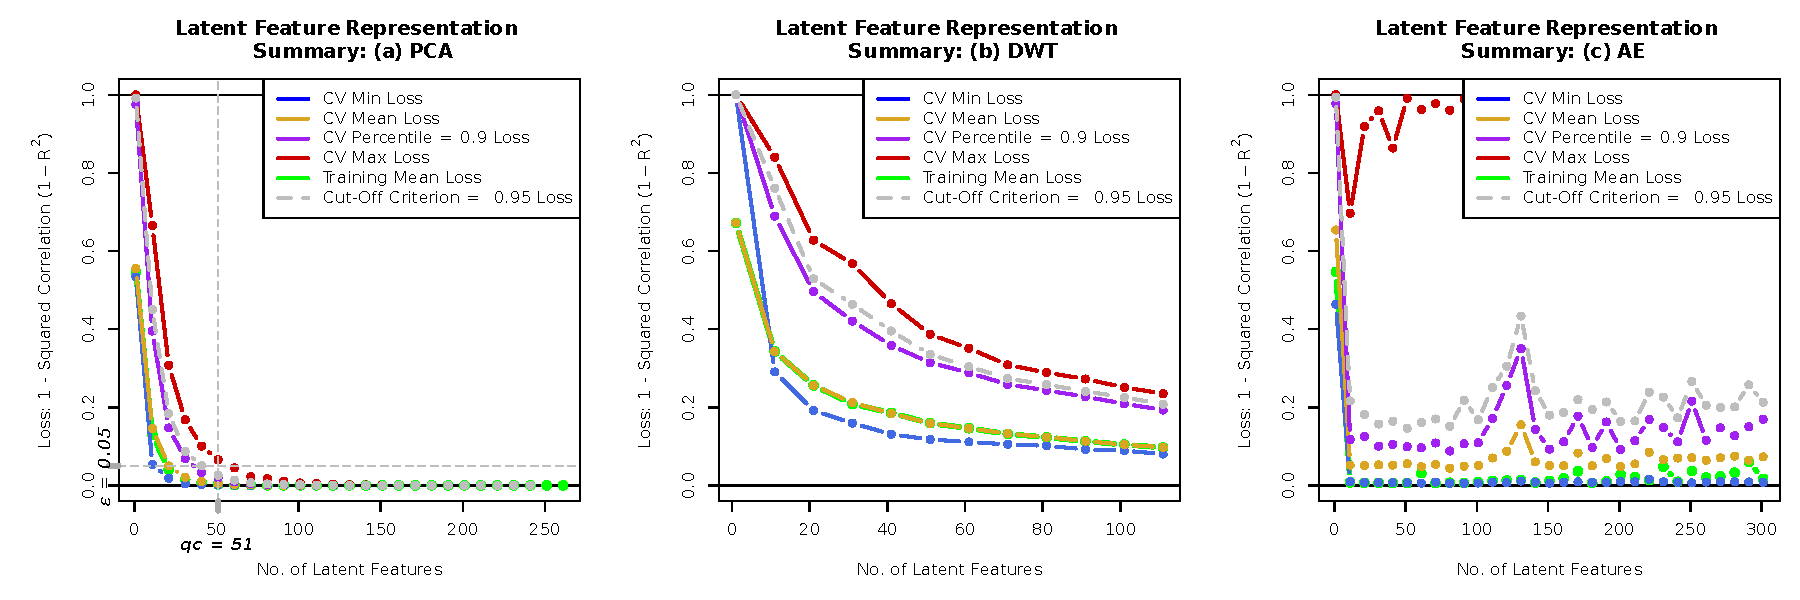
\includegraphics[width=1\textwidth]{figures/eye-results.pdf}
    \caption{Summary \texttt{GLaRe()} plot for the Glaucoma data. A grid of equally-spaced values from $1$ to $261$ in increments of $10$ was used for the latent feature dimensions.}
    \label{fig:eye-results}
\end{figure}

\subsection{Proteomic Gels Data}\label{sec:gels-reults}

\begin{figure}
    \centering
    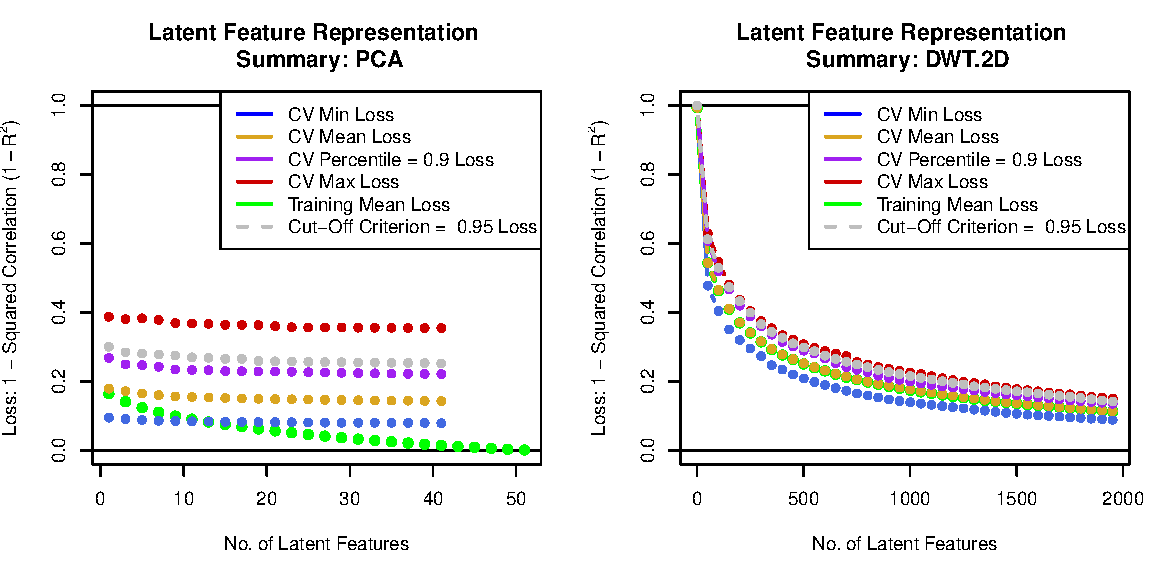
\includegraphics[width=1\linewidth]{figures/initial-gels.pdf}
    \caption{Preliminary results for the gels data.}
    \label{fig:enter-label}
\end{figure}


\subsection{MNIST Digits Data}\label{sec:mnist-reults}

Figure \ref{fig:mnist-results} displays the summary plot from the application of \texttt{GLaRe()} to the MNIST data.
PCA is the most suitable latent feature representation method for this dataset because it achieves the qualifying criterion at $K=201$, whereas DWT achieved it at $K=321$ and the AE did not achieve the qualifying criterion for $K \leq 381$.
A grid of equally-spaced values from $1$ to $381$ in increments of $20$ was used for the latent feature dimensions. 
The computation times for PCA, DWT and AE were $X_1$, $X_2$ and $X_3$ minutes, respectively.

\begin{figure}
    \centering
    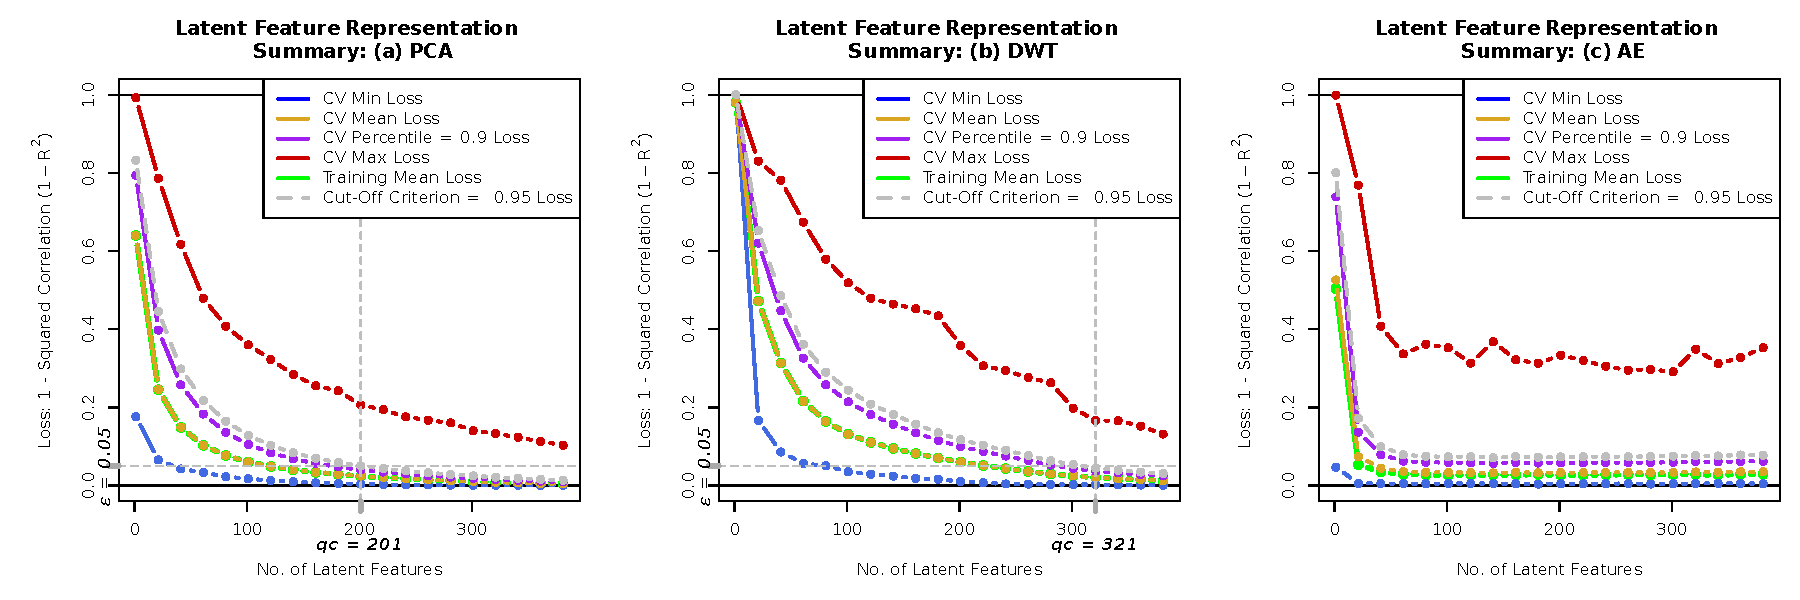
\includegraphics[width=1\textwidth]{figures/mnist-results.pdf}
    \caption{Summary \texttt{GLaRe()} plot for the MNIST data. A grid of equally-spaced values from $1$ to $381$ in increments of $20$ was used for the latent feature dimensions.}
    \label{fig:mnist-results}
\end{figure}

\subsection{Sample Size Experiment}\label{sec:sample-size-experiment}


\begin{figure}
    \centering
    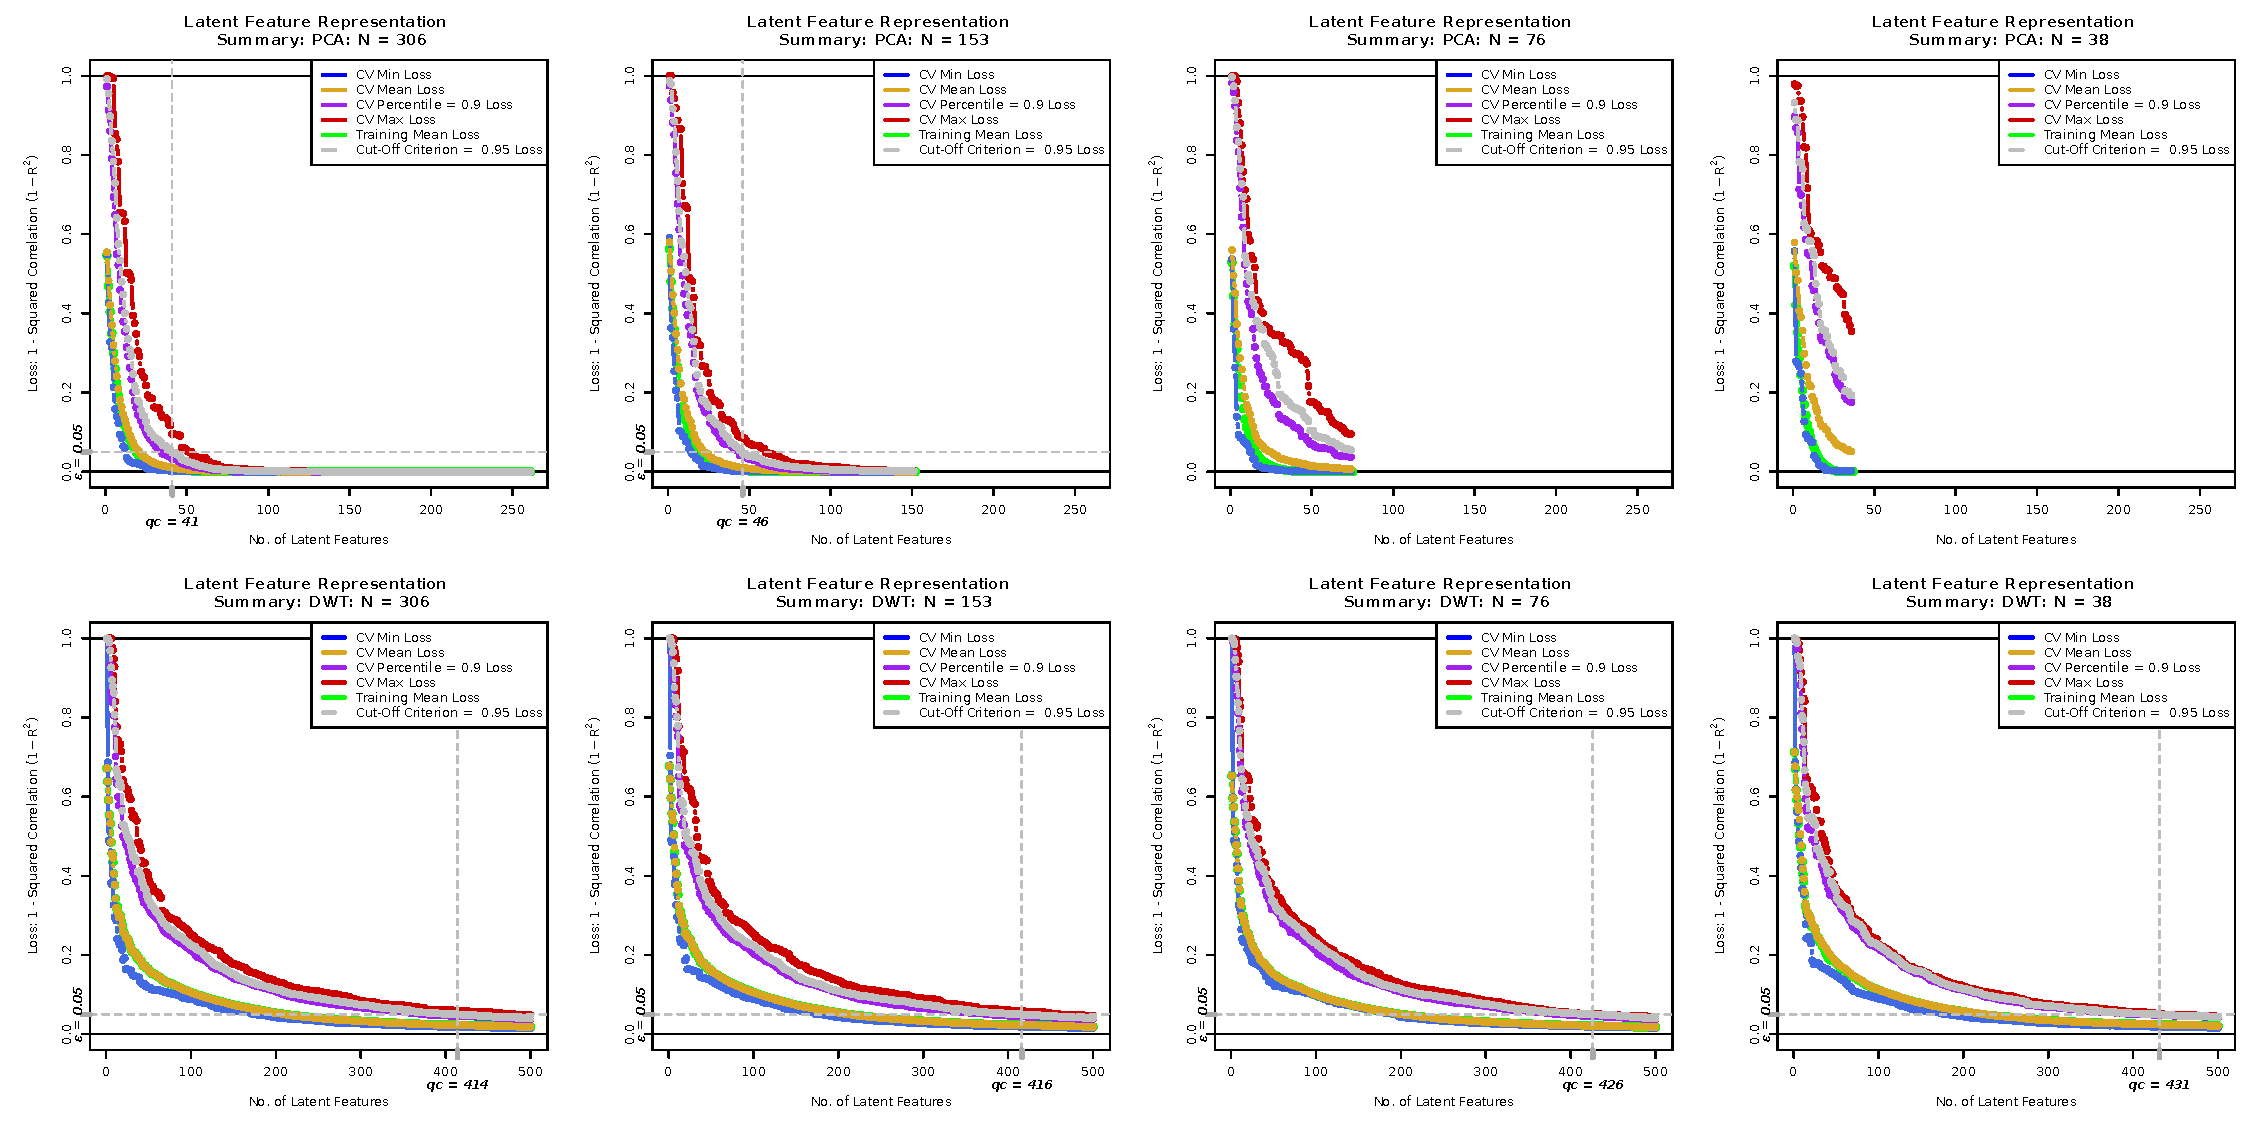
\includegraphics[width=1\linewidth]{figures/eye-sample-size-results-results-01.pdf}
    \caption{Caption}
    \label{fig:eye-sample-size-results-results-01}
\end{figure}


